\documentclass[11pt]{article}
\usepackage{graphicx}
\usepackage[legalpaper,landscape, margin=0.4in]{geometry}
\usepackage{multicol}
\usepackage{titlesec}
\usepackage[dvipsnames]{xcolor}

\titlespacing*{\subsection}
{0pt}{1ex plus 1ex minus .3ex}{0ex}
\titlespacing*{\subsubsection}
{0pt}{1ex plus 1ex minus .3ex}{0ex}
\titleformat{\subsection}
  {\normalfont\fontsize{10.5}{15}\bfseries}{\thesection}{1em}{}
  \titleformat{\subsubsection}
  {\normalfont\fontsize{5}{12}\bfseries}{\thesection}{1em}{}
\begin{document}
\pagenumbering{None}
\setlength{\columnsep}{1cm}
\begin{multicols*}{3}
\section*{CS2107 cheatsheet}\\
{\color{Purple} \rule{\linewidth}{0.5mm} }
\colorlet{link}{RubineRed!70!}
\subsection*{Diffie hellman}
prime and generator is known to everyone\\
Can achieve forward secrecy
\subsection*{Reference monitor}
Order of ACL\\
Check user $>$ member of the group $>$ other
\subsection*{Vulnerability via testing}
White box, black box\\
Fuzzing - send malformed inputs to discover vuln
\\
Accesses to objects: Observe (Read), Alter (Write), Action (Execute)\\
\\
(1)The owner of the object decides the rights. (known as 
discretionary access control)
(2)A system-wide policy decides.  (known as mandatory access 
\subsection*{ Intermediate control}
Fine grain to meet security boundaries that are easy to manage\\
Group - can only by created by root or by a privileged user\\
Role based - determined by the role and assign the permissions for the role (least privilege principle)\\
Protection ring - higher privilege has lower ring number\\
\\
\textrm{\textbf{ Biba and Bell-LaPadula}}\\
Bell lapadula: no read up/ no write down\\
Biba: no write up/ no read down\\
\\
Both: only read/ write to same level\\
\subsection*{Terms}
\textbf{IPSec}
“Internet Protocol Security (IPsec)
communications by authenticating
is a protocol suite for securing Internet Protocol (IP)
and encrypting each IP packet of a communication
session. IPsec includes protocols for establishing mutual authentication \\\\
\textbf{Typosquatting}
Phishing with a typo in domain name leading to attacker's site\\\\
\textbf{Pharming}
poison the dns server and redirects user to a different website that looks the same\\\\
\textbf{Zero day vulnerability}
Use patch to derive vulnerability\\
Known exploits that is released on the day of attack\\\\
\textbf{CVE}
Security vulnerability database\\\\
\textbf{Spamhaus}\\
The Spamhaus Project is an international organisation, based in both London and Geneva, founded in 1998 by Steve Linford to track email spammers and spam-related activity\\\\
\textbf{CERT}\\
Computer Emergency Response Team (CERT) A Computer Emergency Response Team (CERT) is a group of information security experts responsible for the protection against, detection of and response to an organization's cybersecurity incidents\\\\
\textbf{SingCert}\\
Computer Emergency response team\\\\
\textbf{SOC}\\
a centralized unit in an organization that monitors the IT systems and 
deals with security issues\\\\
\textbf{White hat}\\
Access to source code\\
\textbf{Black hat}\\
No access to source code\\
\textbf{Grey hat}\\
Combination of both\\
\subsection*{chmod}
\textcolor{link}{\url{https://www.linode.com/docs/guides/modify-file-permissions-with-chmod/}}\\\\
\textbf{Octal representation}\\
chmod 750[bit for setuid...] ~/example.txt\\
chmod u=rwx,g=rx,o=.\\
setuid (4), setgid (2), and sticky(1)\\
\\
Can also use s to denote setuid\\
runs as the user who owns the executable file instead of the user who invoked the program to access sensitive information\\
\textcolor{link}{https://unix.stackexchange.com/questions/28363/whats-the-difference-between-s-and-s-in-ls-la}\\\\
Effective UID is root is owner is root
\subsection*{ps}
PID 1 is actively reserved for the init process to maintain consistency with older systems\\
\textcolor{link}{https://en.wikipedia.org/wiki/Process\_identifier}\\
\subsection*{Linux file permissions}
drwxr-xr-x\\
first character indicates whether it is a file or directory\\
Date is the date of last modification
\subsection*{Buffer overflow}\\
\%p points to a pointer (address)\\
\subsection*{Hash functions}
SHA256 needs to protect both the public key and private key
\subsection*{Birthday attack}
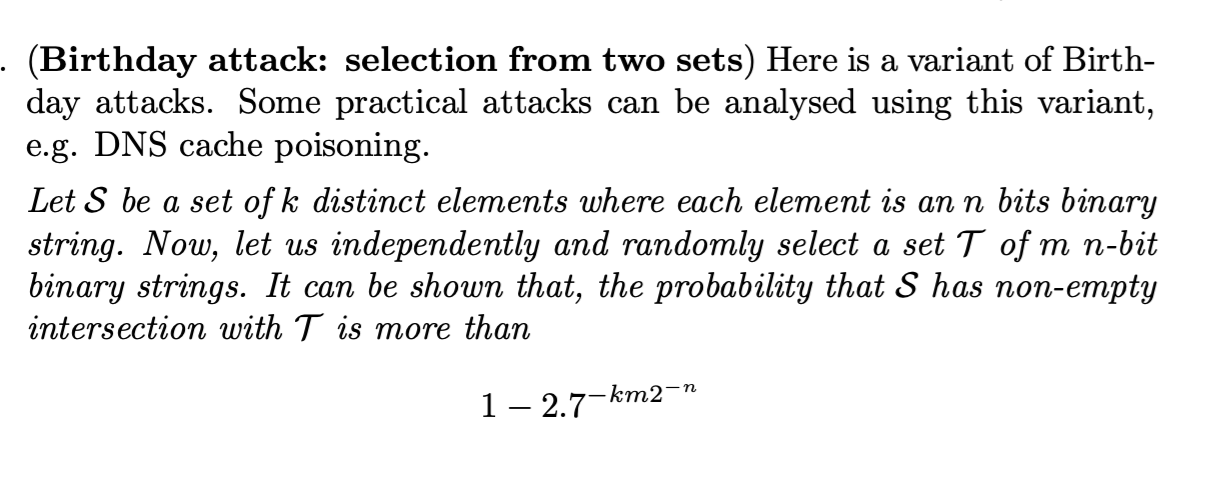
\includegraphics[height=3cm]{ss1}
\\
M $>$ 1.17 \sqrt{T}
\subsection*{Unilateral Authentication}
Generates a session key pair $<$k, t$>$ by verify the authenticity using the entity's public key\\\\
Related: MiTM,\\
When message is sent from Alice to Bob, decrypt using $k_{a}$ and encrypt using $k_{b}$\\
\subsection*{Strong Authentication - Challenge/Response}
Use shared secret key to generate mac, verification on receipt
\subsection*{Nonce}
Random number used in unilateral authentical using PKC to prevent replay attacks\\
Record everything and replay what the attacker has seen before\\
64-bit is more than sufficient to prevent the attacker from seeing a repeated nonce, need to observe large number of historical communication
\subsection*{Certificate Structure}
(i) Name of an entity \\
(ii) Public key \\
(iii) Expiry data \\
(iv) Signature\\\\
\textbf{Self signed certificate}\\
Signed using entity's private key\\\\
\textbf{Encryption - Stream Cipher}\\
AES Counter mode\\\\
$msg_{0}$ and $mac_{0}$ \\
$ mac_{0}$ = (IV $\|$ xor cipher)\\
$mac_{1}$ can be forged with (IV $\|$ xor cipher XOR H(msg))\\\\
\textbf{RSA}\\
Subjected to factorization search is e is  65536 and below\\\\
\textbf{Renegotiable attack - TLS}\\
Client is connected to attacker server that connects with the actual server\\
Can be mitigated using CSRF\\
Key for the first handshake encrypts the second handshake\\
Does not compromise confidentiality\\
Disabling renegotiation affects availability
\\\\
\textbf{XSS}\\
\textcolor{link}{https://owasp.org/www-community/xss-filter-evasion-cheatsheet}\\\\
\textbf{Kerckhoff ’s principle}\\
adversaries know the
algorithm and format of the token\\
Replace with MAC
\\\\
\subsection*{RFC4086 recommendations}\\
Password At least 30 bits to be secure against online attacks, 60 bits against offline attacks \\
\subsection*{NIST recommendations}\\
Password 128 bits against offline attacks 
\subsection*{Cracking Dmgs}
\textcolor{link}{https://www.whitehatsec.com/blog/cracking-aes-256-dmgs-and-epic-self-pwnage/}
\\
\subsection*{Compiling source code}
John the ripper can crack /etc/shadow, break dmg\\
\textcolor{link}{https://dfir.science/2014/07/how-to-compiling-john-ripper-to-use-all.html}\\
\\./dmg2john your\_file.dmg $>>$ output
\\./john output]\\
or ./john - -format=dmg-opencl output\\
\\
View Makefile.in using nano, it asks to run with ./configure && make\\
\textcolor{link}{https://stackoverflow.com/questions/30805803/how-to-create-link-to-directory-in-makefile-in-linux}\\
\\
Can find more of the commands for pen test here\\
\textcolor{link}{https://www.hackingarticles.in/category/penetration-testing/}
\subsection*{Heartbleed bug}\\
Send more than the length of the request
\textcolor{link}{https://www.csoonline.com/article/3223203/what-is-the-heartbleed-bug-how-does-it-work-and-how-was-it-fixed.html}
\subsection*{WPA2}
Variants of WPA2, LEAP and PEAP (safe against offline attacks, but not online attacks)\\\\
Happens at link and physical layer\\
Key reinstallation attack bypasses https with sslstrip protocol\\
Github allows attacker to bypass firewall\\\\
If communication is carried out, the person is not aware that communication has occured\\
Covert channel hides the communication as the attacker doesn't want others to know that the machine is compromised
\\\\
TLS protect app information, WiFi protect the routing information\\
Attacker unable to spoof the IP address with IPSec, can only know source and destination (need to modify OS)\\
IP address may not be unique on the web server, but it is not a problem as there is a subnet\\\\
HTTP is built on top of TLS, SSL is the predecessor of TLS
\end{multicols*}

\end{document}
